%!TEX root =  main.tex
\section{\dynastar: dynamic and quasi-optimum state partitioning}
%\section{\dynastar: dynamic partitioning for scalable state machine replication}
%\section{The centralized partitioning scheme}

%If the system can be modeled as a graph, as described in the previous session, we can take advantage of algorithms that perform graph partitioning to optimise the state partitioning of \ssmr\  while using concepts from \dssmr. The problem of graph partitioning is well stablished and despite being NP-Complete \ref{NPC_GraphPartition}, several approximation algorithms exist. First we define what graph partitioning is and how it can analyzed to our needs, next we explore possibilities that are easily obtainable when applying the same graph's reasoning.

\subsection{Overview}
%\subsection{State partitioning as a graph problem}

We represent a service workload as a graph $G = (V, E)$, where vertices are state objects and an edges are operations.
There is an edge connecting two objects in the graph if a client can issue a command that accesses the objects. 




\subsection{The \dynastar protocol}

Algorithms~\ref{alg:client_proxy}, \ref{alg:server_proxy}, and \ref{alg:oracle_proxy} describe in detail how client, server and oracle processes execute, respectively.
For brevity, we omit the delete command since the coordination involved in the execution of a create and of a delete commands are analogous. 
Moreover, in the discussion in this section, every command involves the oracle.
In the next section, we explain how clients can use a caching technique to avoid using the oracle in the execution of most commands.

\begin{figure*}
\begin{minipage}[b]{1\linewidth} % A minipage that covers the whole width of the page
\centering
      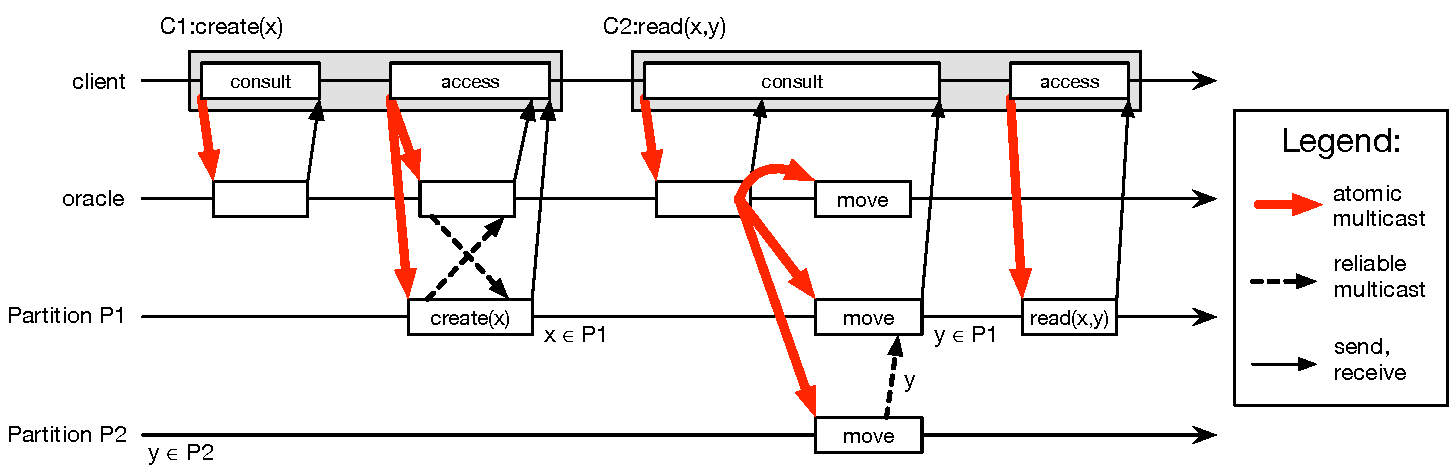
\includegraphics[width=0.9\linewidth]{figures/dynastar}
\end{minipage}
\caption{The execution of a create command and a read command in \dynastar.}
\label{fig:oracle_repartition}
\end{figure*}

%When issuing a command, the application simply forwards the command to the client proxy and waits for the reply.
%Consulting the oracle and multicasting the command to different partitions is done internally by the proxy at the client.
%Every server proxy at a server in $\ssm_i$ has only partial knowledge of the partitioning: it knows only which variables belong to $\ppm_i$.
%The oracle proxy has knowledge of every $\ppm \in \Psi$.
%To maintain such a global knowledge, the oracle must \amdel{} every command that creates, moves, or deletes variables.
%(In Section~\ref{sec:optm}, we introduce a caching mechanism to prevent the oracle from becoming a performance bottleneck.)

%\clearpage
\begin{algorithm}[h!]
\small

\begin{distribalgo}[1]

\vspace{1.0mm}

\INDENT{To issue a command $C$, the client proxy does:}

\vspace{1.0mm}

    \INDENT{\textbf{do}}
        \STATE \amcast$($oracle, $consult(C))$
        \STATE wait for $prophecy$
        \IF{$prophecy \in \{ok, nok\}$}
            \STATE $reply \leftarrow prophecy$
        \ELSE
            \STATE $C.vars \leftarrow \{v: \exists P : \langle v, P \rangle \in prophecy \}$
            \STATE $C.dests \leftarrow \{P: \exists v : \langle v, P \rangle \in prophecy \}$
            \IF{$C$ is an $access$ command and $|C.dests| > 1$}
                \STATE let $P_d$ be one of the partitions in $C.dests$
                \FOR{every $v \in C.vars$}
                    \STATE // \textit{move $v$ partition $P_d$}
                    \STATE let $P_o$ be $P : \langle v, P \rangle \in prophecy$
                    \IF{$P_o \neq P_d$}
                        \STATE $C_{move} \leftarrow move(v,P_d)$
                        \STATE $C_{move}.dests \leftarrow \{$oracle$,P_o,P_d\}$    
                        \STATE \amcast$(C_{move}.dests$, $C_{move})$
                    \ENDIF
                \ENDFOR
                \STATE $C.dests \leftarrow \{ P_s \}$
            \ENDIF
            \IF{$C$ is $create$ or $delete$}
                \STATE $C.dests \leftarrow dests \cup \{oracle\}$
            \ENDIF
            \STATE \amcast$(C.dests$, $C)$
            \STATE wait for $reply$
        \ENDIF
    \ENDINDENT
    \STATE{\textbf{while} $reply = retry$ // \textit{after $n$ retries, fall back to \ssmr}}
    \STATE return $reply$ to the application client
\ENDINDENT

\caption{\dssmr\ Client Proxy}
\label{alg:client_proxy}
\end{distribalgo}
\end{algorithm}
\begin{algorithm}[h!]
\small

\begin{distribalgo}[1]

\vspace{1.0mm}

\INDENT{To execute a command $C$, the server proxy in partition $\ppm$ does:}

    \vspace{1.0mm}
    
    \INDENT{\textbf{when} \rmdel$( \langle val, C \rangle )$}
        \STATE $rcvd\_msgs \leftarrow rcvd\_msgs \cup \{\langle val, C \rangle\}$
    \ENDINDENT

    \vspace{1.0mm}

    \INDENT{\textbf{when} \amdel$(C)$}

    \vspace{1.0mm}

        \IF{\underline{$C$ is an $access(\omega)$ command}}
            \IF{$\exists v \in \omega : v \not\in \ppm$}
                \STATE reply with $retry$
            \ELSE
                \STATE have the command executed by the application server
                \STATE send the reply to the client
            \ENDIF
        

        \vspace{1.0mm}
    
        \ELSIF{\underline{$C$ is a $move(v,\ppm_s,\ppm_d)$ command}}
            \IF{$\ppm = \ppm_s$}
                \IF{$v \in \ppm$}
                    \STATE \rmcast$(\ppm_d$,$\langle v, C \rangle)$
                    \STATE $\ppm \leftarrow \ppm \setminus \{v\}$
                \ELSE
                    \STATE \rmcast$(\ppm_d$,$\langle null, C \rangle)$
                \ENDIF
            \ELSE
                \STATE wait until $\exists val : \langle val, C \rangle \in rcvd\_msgs$
                \IF{$val \neq null$}
                    \STATE $v \leftarrow val$
                    \STATE $\ppm \leftarrow \ppm \cup \{v\}$
                \ENDIF
            \ENDIF
        
        \vspace{1.0mm}
    
        \ELSIF{\underline{$C$ is a $create(v)$ command}}
            \STATE wait until $\langle val, C \rangle \in rcvd\_msgs$
            \IF{$val = ok$}
                \STATE $\ppm \leftarrow \ppm \cup \{v\}$
%                \STATE reply with $success$
%            \ELSE
%                \STATE reply with $retry$
            \ENDIF
        
        \vspace{1.0mm}
        
        \ELSIF{\underline{$C$ is a $delete(v)$ command}}
            \IF{$v \in \ppm$}
                \STATE $\ppm \leftarrow \ppm \setminus \{v\}$
%                \STATE reply with $success$
%            \ELSE
%                \STATE reply with $retry$
            \ENDIF
        \ENDIF
    \ENDINDENT
\ENDINDENT

\caption{\dssmr\ Server Proxy}
\label{alg:server_proxy}
\end{distribalgo}
\end{algorithm}
\begin{algorithm}[t!]
\small

\begin{distribalgo}[1]

%\vspace{1.0mm}

	\INDENT[\textbf{Task 1}]{\colorbox{\coloralgo}{\textbf{when} \amdel$(consult(C))$}}
%		\INDENT{\textbf{case} $C$ is a $consult(C_c)$ command:}
%			\STATE $update(G_W, \omega)$
			\INDENT{\textbf{case} $C$ is a $create(v)$ command:}
				\IF[if $v$ already exists...]{$\parts(\{v\}) \neq \bot$}
					\STATE $prophecy \leftarrow nok$
					\COMMENT{...notify client}
				\ELSE[if $v$ doesn't exist...]
					\STATE $\ppm \leftarrow target(G_W, \{v\})$
					\COMMENT{...determine $v$'s partition}
					\STATE $prophecy \leftarrow (\{ \ppm, oracle \}, false)$
%					\COMMENT{prepare client's response}
				\ENDIF
			\ENDINDENT
			\INDENT{\textbf{case} $C$ is an $access(\omega)$ command:}
				\IF[if $v$ doesn't exist:]{$\exists v \in \omega : \parts(\{v\}) = \bot$}
					\STATE $prophecy \leftarrow nok$
					\COMMENT{tell the client}
				\ELSE[if all vars in $\omega$ exist]
%					\STATE $dests \leftarrow \emptyset$
%					\FOR{each $v \in \omega$}
%						\STATE $dests \leftarrow dests \cup partition(v)$
%					\ENDFOR
					\STATE $dests \leftarrow \parts(\omega)$
					\COMMENT{get all partition involved}
					\IF[if only one partition:]{$|dests| = 1$}
						\STATE $prophecy \leftarrow (dests,false)$
%						\COMMENT{tell client which partition}
					\ELSE[if multiple partitions involved]
						\STATE $\ppm_d \leftarrow target(G_W, \omega)$
						\COMMENT{$\ppm_d$ will store all vars in $\omega$}
						\STATE $alldest \leftarrow \{oracle\} \cup dests$
						\COMMENT{move $v$ from $\ppm_s$...}
						\STATE \amcast$(alldest, move(\omega,dests,\ppm_d))$
						\COMMENT{...to $\ppm_d$}						
%						\FOR[for each involved var $v$]{each $v \in \omega$}
%							\STATE $\ppm_s \leftarrow \parts(\{v\})$
%							\COMMENT{$\ppm_s$ is $v$'s current partition}
%							\IF[if $v$ not in $\ppm_d$:]{$\ppm_s \neq \ppm_d$}
%								\STATE $aux \leftarrow \{oracle,\ppm_s,\ppm_d\}$
%								\COMMENT{move $v$ from $\ppm_s$...}
%								\STATE \amcast$(aux$, $move(v,\ppm_s,\ppm_d))$
%								\COMMENT{...to $\ppm_d$}
%							\ENDIF 
%						\ENDFOR
						\STATE $prophecy \leftarrow (\{\ppm_d\},true)$
					\ENDIF 
				\ENDIF
			\ENDINDENT
			\STATE send $prophecy$ to the client
%			\INDENT{\textbf{case} $C_c$ is a $delete(v)$ command:}
%				\IF{$partition(v) = \bot$}
%					\STATE $prophecy \leftarrow ok$
%				\ELSE
%					\STATE $prophecy \leftarrow (\{ \ppm : v \in \ppm, oracle \}, -)$
%				\ENDIF
%			\ENDINDENT
%		\ENDINDENT
	\ENDINDENT
	\vspace{1.0mm}

	\INDENT[\textbf{Task 2}]{\colorbox{\coloralgo}{\textbf{when} \amdel$(create(v))$}}
%	\INDENT{\textbf{case} $C$ is a $create(v)$ command:}
		\STATE let $\ppm_c \in C.dests \setminus \{oracle\}$
		\COMMENT{var created in $\ppm_c$}
		\STATE \rmcast$(\ppm_c, \langle signal, C \rangle )$
		\COMMENT{exchange signal to...}
		\STATE wait until $\langle signal, C \rangle \in rcvd\_msgs$
		\COMMENT{...coordinate partitions}
		\STATE $\ppm_c \leftarrow \ppm_c \cup      \{v\}$
                \STATE send $ok$ to the client
	\ENDINDENT

	\vspace{1.0mm}
	\INDENT[\textbf{Task 3}]{\colorbox{\coloralgo}{\textbf{when} \amdel$(move(\omega,dests,\ppm_d))$}}
%        \INDENT{\textbf{case} $C$ is a $move(v,\ppm_s,\ppm_d)$ command:}
                \STATE \textbf{for} each $\ppm_s \in dests$ \textbf{do} $\ppm_s \leftarrow \ppm_s \setminus \omega$
                \COMMENT{update partitions...}
                \STATE $\ppm_d \leftarrow \ppm_d \cup \omega$
                \COMMENT{...and add new variables}
                \STATE send $ok$ to the client
	\ENDINDENT

        \vspace{1.0mm}
    
	\INDENT[\textbf{Task 4}]{\colorbox{\coloralgo}{\textbf{when} \rmdel$( \langle val, C \rangle )$}}
		\STATE $rcvd\_msgs \leftarrow rcvd\_msgs \cup \{\langle val, C \rangle\}$
	\ENDINDENT
	
	\vspace{1.0mm}
	\INDENT{\colorbox{\coloralgo}{\textbf{function} \parts$(vars)$}}
		\STATE $aux \leftarrow \{ \ppm : \exists v \in vars \cap \ppm \}$
		\STATE return $aux$
	\ENDINDENT
	
%	\vspace{1.0mm}
	\rule{83mm}{0.4pt}
%	\vspace{0.1mm}

	\INDENT[\textbf{Task 5}]{\colorbox{\coloralgo}{\textbf{when} \amdel$(hint(V_h,E_h))$}}
		\STATE update $G_W$ with $(V_h,E_h)$
%		\STATE send $ok$ to the client
	\ENDINDENT
	
	\vspace{1.0mm}
    
	\INDENT[\textbf{Task 6}]{\colorbox{\coloralgo}{\textbf{periodically} do}}
		\STATE compute ideal partition $\ip_1, ..., \ip_m$ from $G_W$
	\ENDINDENT
	
	\vspace{1.0mm}
    
	\INDENT{\colorbox{\coloralgo}{\textbf{function} target$(vars)$}}
		\STATE $\ppm \leftarrow$ compute destination partition for $vars$ from\\ \hspace{8mm}current $\ppm_1, ..., \ppm_m$ and ideal $\ip_1, ..., \ip_m$ partitionings
		\STATE return $\ppm$
	\ENDINDENT	
	
%	\vspace{1.0mm}
%        
%	\INDENT{\textbf{case} $C$ is a $delete(v)$ command:}
%		\STATE let $\ppm_d$ be $\ppm : \{\ppm\} = C.dests \setminus \{$oracle$\}$
%		\STATE $\ppm_c \leftarrow \ppm_c \setminus      \{v\}$
%		\STATE \rmcast$(\ppm_c, \langle ok, C \rangle )$
%			\STATE wait until $\exists val : \langle val, C \rangle \in rcvd\_msgs$
%	\ENDINDENT

%\ENDINDENT

\caption{Oracle}
\label{alg:oracle_proxy}
\end{distribalgo}
\end{algorithm}



\subsubsection{The client process} 

To execute a command $C$, the client atomically multicasts $C$ to the oracle in a consult message to find out the partitions involved in $C$.
The oracle replies with a prophecy, which may already tell the client that $C$ cannot be execute (e.g., $C$ needs a variable that does not exist, $C$ tries to create a variable that already exists).
If the command can be executed, the client receives a prophecy containing a tuple $(dests, sync)$, where $dests$ is a set of the partitions the command must be atomically multicast to for execution, and $sync$ is a set with the partitions the client must coordinate with before multicasting the command.
The client must coordinate with partitions before atomically multicasting a command if the command involves variables located in multiple partitions and the oracle needs to move variables to a single partition (in which case $sync$ contains the partitions involved in the moves).

After the client atomically multicasts $C$ to the target partition, it waits for a response from the servers in the target partition.
The client must retry the command if the target partition cannot execute the command.
This happens if some of the variables needed by $C$ were moved to another partition due to the interleaving of $C$ with other commands. 
To ensure that command $C$ is eventually executed, after retrying a few times, the client falls back \ssmr{}, multicasting $C$ to all partitions (and the oracle, in case $C$ is a create or delete command).

\subsubsection{The server process} 

When a server delivers a command for execution, it first checks that all variables accessed by the command are stored locally, in which case the command is executed and the response is sent back to the client (Task 1 in Algorithm~\ref{alg:server_proxy}).
If one or more variables are not stored at the partition, the server returns a message to the client to retry the operation.
This happens if some variables have been moved to another partition due to another command. 

Upon delivering a message to move variable $v$ (Task 2), a server in the source partition checks whether $v$ is still stored locally, in which case the server reliably multicasts $v$ to the destination partition; if $v$ is no longer stored in the partition, the server sends a null message to the destination partition.
Servers in the destination partition simply wait for a message from the source partition.

When a server delivers a message to create a variable (and similarly to delete an existing variable), it coordinates with the oracle (Task 3).
The exchange of signals between the partition where the variable will be created and the oracle ensures that interleaved executions between create and delete commands will not lead to violations of linearizability.

\subsubsection{The oracle process} 

One of the purposes of the oracle proxy is to make prophecies regarding the location of state variables.
Such prophecies are used by client proxies to multicast commands to the right partitions.
A prophecy regarding an $access(\omega)$ command contains, for each $v \in \omega$, a pair $\langle v, \ppm \rangle$, meaning that $v \in \ppm$.
If any of the variables in $\omega$ does not exist, the prophecy already tells the client that the command cannot be executed (with a $nok$ value).
For a $create(v)$ command, the prophecy tells where $v$ should be created, based on rules defined by the application, if $v$ does not exist.
If $v$ already exists, the prophecy will contain $nok$, so that the client knows that the create command cannot be executed.
The prophecy regarding a $delete(v)$ command contains the partition that contains $v$, or $ok$, in case $v$ was already deleted or never~existed.

Besides dispensing prophecies, the oracle is responsible for executing create, move, and delete commands, coordinating with server proxies when necessary, and replying directly to clients in some cases.
For each $move(v,\ppm_s,\ppm_d)$ command, the oracle checks whether $v$ in fact belongs to the source partition $\ppm_s$.
If that is the case, the command is executed, moving $v$ to $\ppm_d$.
Each $create(v)$ command is multicast to the oracle and to a partition $\ppm$.
If $v$ already exists, the oracle tells $\ppm$ that the command cannot be executed, by \rmcast{}ing $nok$ to $\ppm$.
The oracle also sends $nok$ to the client as reply, meaning that $v$ already exists.
If $v$ does not exist, the oracle tells $\ppm$ that the command can be executed, by \rmcast{}ing $ok$ to $\ppm$.
It also tells the client that the command succeeded with an $ok$ reply.
Finally, each $delete(v)$ command is multicast to the oracle and to a partition $\ppm$, where the client proxy assumed $v$ to be located.
If $v$ belongs to $\ppm$, or $v$ does not exist, the oracle tells the client that the delete command succeeded.
Otherwise, that is, if $v$ exists, but $delete(v)$ was multicast to the wrong partition, the oracle tells the client to retry.



\subsection{Performance optimizations}
\label{sec:optm}

In this section, we introduce two optimizations for \dssmr{}: caching and load balancing.

In Algorithm~\ref{alg:client_proxy}, for every command issued by the client, the proxy consults the oracle.
If every command passes by the oracle, the system is unlikely to scale, as the oracle is prone to becoming a bottleneck.
To provide a scalable solution, each client proxy has a local cache of the partitioning information.
Before multicasting an application command $C$ to be executed, the client proxy checks whether the cache has information about every variable concerned by $C$.
If the cache does have such a knowledge, the oracle is not consulted and the information contained in the cache is used instead.
If the reply to $C$ is $retry$, the oracle is consulted and the returned prophecy is used to update the client proxy's cache.
Algorithm~\ref{alg:client_proxy} is followed from the second attempt to execute $C$ on.
The cache is a local service that follows an algorithm similar to that of the oracle, except it responds only to $consult(C)$ commands and, in situations where the oracle would return $ok$ or $nok$, the cache tells the client proxy to consult the actual oracle.

Naturally, the cached partitioning information held by the client proxy may be out of date.
On the one hand, this may lead a command to be multicast to the wrong set of partitions, which will probably incur in the client proxy having to retry executing the command.
For instance, in Figure~\ref{fig:cache_retry} the client has an out-of-date cache, incurring in a new consultation to the oracle when executing $C_3$.
On the other hand, the client proxy may already have to retry commands, even if the oracle is always consulted first, as shown in Figure~\ref{fig:move_case_1}.
If most commands are executed without consulting the oracle, as in the case of $C_4$ in Figure~\ref{fig:cache_retry}, we avoid turning the oracle into a bottleneck.
Moreover, such a cache can be updated ahead of time, not having to wait for an actual application command to be issued to only then consult the oracle.
This way, the client proxy can keep a cache of partitioning information of variables that the proxy deems likely to be accessed in the future.




\subsection{Correctness}
\label{sec:correctness}

In this section, we argue that \dssmr\ ensures termination and linearizability.
By ensuring termination, we mean that for every command $C$ issued by a correct client, a reply to $C$ different than $retry$ is eventually received by the client.
This assumes that at least one oracle process is correct and that every partition has at least one correct server.
Given these constraints, the only thing that could prevent a command from terminating would be an execution that forced the client proxy to keep retrying a command.
This problem is trivially solved by falling back to \ssmr\ after a predefined number of retries: at a certain point, the client proxy multicast the command to all server and oracle processes, which execute the command as in \ssmr{}, i.e., with coordination among all partitions and the oracle.

As for linearizability, we argue that, if every command in execution \ex\ of \dssmr\ is delivered by atomic multicast and is \emph{execution atomic} (as defined in~\cite{bezerra2014ssmr}), then \ex\ is linearizable.
We denote the order given by atomic multicast by relation $\prec$.
Given any two messages $m_1$ and $m_2$, ``$m_1 \prec m_2$'' means that there exists a process that delivers both messages and $m_1$ is delivered before $m_2$, or there is some message $m'$ such that $m_1 \prec m'$ and $m' \prec m_2$, which can be written as \mbox{$m_1 \prec m' \prec m_2$}.
%\fxnote[draft]{use the phrase \"there exists a process that\" }
Also, for the purposes of this proof, we consider the oracle to be a partition, as it also \amdel{}s and executes application commands.

Suppose, by means of contradiction, that there exist two commands $x$ and $y$, where $x$ finishes before $y$ starts, but $y \prec x$ in the execution.
There are two possibilities to be considered: (i) $x$ and $y$ are delivered by the same process $p$, or (ii) no process delivers both $x$ and $y$.

In case (i), at least one process $p$ delivers both $x$ and $y$.
As $x$ finishes before $y$ starts, then $p$ delivers $x$, then $y$. From the properties of atomic multicast, and since each partition is mapped to a multicast group, no process delivers $y$, then $x$.
Therefore, we reach a contradiction in this case.

In case (ii), if there were no other commands in \ex, then the execution of $x$ and $y$ could be done in any order, which would contradict the supposition that $y \prec x$.
Therefore, there are commands $z_1, ..., z_n$ with atomic order $y \prec z_1 \prec \cdots \prec z_n \prec x$, where some process $p_0$ (of partition $\ppm_0$) delivers $y$, then $z_1$; some process $p_1 \in \ppm_1$ delivers $z_1$, then $z_2$, and so on: process $p_i \in \ppm_i$ delivers $z_{i}$, then $z_{i+1}$, where $1 \leq i < n$.
Finally, process $p_n \in \ppm_n$ delivers $z_n$, then $x$.

Let $z_0 = y$ and let $atomic(i)$ be the following predicate:
``For every process $p_i \in \ppm_i$, $p_i$ finishes executing $z_i$ only after some $p_0 \in \ppm_0$ started executing $z_0$.''
We now claim that $atomic(i)$ is true for every $i$, where $0 \leq i \leq n$.
We prove our claim by induction.





